\chapter{Data processing}
STORM data from different cells or structures show many different features, there can be clusters of flourophores with a high density of spots, low density, variable background in space and time, beads can be present or not. This section is about how the algorithm processes the data sets and how it is possible to find good settings that will work for all kind of input data. 


\section{Import and processing}
The STORM data has usually a size of around 3 gigabyte. There are even larger datasets possible, so that it is important to work on smaller parts of the data, instead putting the whole dataset into memory. This is done using chunks of user defined size. The data is processed chunkwise, there is parallelisation for the frames of each chunk. This is possible because the signals in each frame are considered to be independent from each other.  

\section{Workflow}
\subsection{Chose parameters}
At the begining the user has the option to set all important parameters, if no parameter is set the default ones are used and will give a good result because all crucial parameters are either determined from the data or set to reasonable values that work for every data set. The focus of the default parameters is to give a good result with no adjustment. This means parameters are chosen to produce almost 100 \% precission. The loss of some points that are not detected using this conservative setting won't affact the final result as much as a lower precission will do.
\subsection{Estimating camera gain and offset}
First of all it is checked whether there exists a file containing settings for gain and offset from an earlier run. If this is not the case new parameters are estimated based on the first part of the data, usually 200 frames are sufficiant.\newline
The method described by \cite{skellam} is used to estimate the
gain factor. For this methode a Skellam distribution is used. 
Each dataset is three-dimensional where time is the third
dimension. Therefore mean $\mu$ and variance $\sigma^2$, in time, can be calculated from
the data for each pixel individually
\begin{align}
	\mu(i,j) & = \frac{\Sigma_t(I_t(i,j)-I_{t+1}(i,j))}{n}\\
	\sigma^2 & = \frac{\Sigma_t(\mu-(I_t(i,j)-I_{t+1}(i,j)))^2}{n-1}
\end{align} 
To determine the gain factor the Skellam parameter are plotted over the mean
intensities. A straight line can be fitted and its slope gives the gain
factor.
\subsection{Recursively adjusting gain and offset}
After the estimation of gain factor and offset, the transformations described in \ref{trafoPoiss} and \ref{trafoAnscombe} are applied and the background subtracted.\newline
Due to the Anscombe transformation the background pixels of the image should only vary around a mean intensity of zero with a variance of 1. Therefore a histogramm of the pixel intensities is created. The after background subtraction the background pixels should contribute only to the lower intensities in the histogramm. A gaussian function is fitted to the histogramms values. This is done under the assumption that there is much more background in the image than signal or the intensities coming from signals are distributed over a larger range, so the gaussian for the background intensity distribution can be fitted correctly.\newline
If the estimated value for the variance is too far off 1 the originally estimated gain factor is corrected, applied and the fit is done again. This is done until the background variance converges or the maximal number of iterations is reached. In this case the initial gain factor will be used and a warning printed to the screen.
\subsection{Estimating the width of the point spread function}
For a certain number of frames the Fourier transform is calculated and averaged. The result is called mean power spectrum. It can be used to estimate the variance of the point spread function of the signal. A two dimensional gaussian functions Fourier transform is again a gaussian but with inverse variance. This relation is used to determine the variance of the point spread function in spatial domain, using the fit parameter for the variance in frequency domain.
\subsection{Processing the data}
\subsubsection{Import Data}
Storm data sets can consist of several thousand frames with resolutions up to one mega pixel per frame. This makes it necessary to break the data into smaller parts because otherwise it might be much larger as the RAM of an ordinary machine. Because of the background estimation it is not possible to process every frame completly independent as it was in the older version of this software \cite{MAJoachim}. It is also faster with some datatypes to load a larger consecutive part of the dataset into memory.\newline
This algorithm uses chunks of user defined size. There are some limitations to the chuncksize that are discussed later. The data set is split into parts of equal size in $x$- and $y$-dimensions and independently also in $t$-dimension. If this partition does not fit at the edge of the data set, the last chunks will be smaller.\newline
The data is transformed to be Poission distributed and after that the Anscombe transform is applied.
\subsubsection{Background estimation}
For each chunk the median is determined to get a robust estimate of the background value for this chunk. 
The Bspline interpolation implemented in vigra \cite{vigra} is used to get interpolated values for the full resolution of the current frames. For this interpolation three chunks in $t$-dimension have to be available. Therefore the maximal chunksize in $t$-dimension must not be larger than a third of the total stacksize.\newline
This background is then subtracted from the transformed data to give finally background pixels with zero mean and a variance of one, both in $xy$- and in $t$-dimension.
\subsubsection{Create mask for background suppression}
With the given $p$-value from the settings a global threshold can be determined, because inhomogeneities of background intensities has been removed. The threshold value is that intensity that is explained from a gaussian distribution with mean zero and variance one with the given $p$ probability. This is possible because the background intensity follows such a distribution after all the applied transformations.\newline
The threshold is applied to the current frame and stored as a mask. Due to the probability that background pixels intensitis might exceed the threshold the connected components of the mask are calculated. Pixels that belong to connected components with too few members are discarded. 
\subsubsection{Filter data and finding maxima}
To imporve the accuracy of the spot detection the transformed signal is convolved with a two dimensional gaussian function with the previously determined or user set width. The convolved image will further be used to find the maxima. Each maxima found is tested to be covered by the mask or discared otherwise. A region of intrest around the remaining maxima is interpolated to a higher resolution. In the interpolated region  it is searched for maxima for the last time. This maxima will be detected with super resolution.\\
To determin the signal-noise-ratio the unfilterd and uninterpolated pixelintensity is used.

\subsubsection{Quality control for detections}
Especially in data sets with a high density of spots it can happen, that two spots are near each other and the point spread functions overlap. It may happen that instead of two maxima just one maximum will be detected right between the true ones. This leads to large errors in the localisation. To avoid this a threshold for the asymmetry of the spots can be set.


\section{Comparison with older version of the storm algorithm}
\subsection{Adjustable filter width}
\subsection{Treatment of variable background}



\section{New graphical user Interface (GUI)}
\subsection{Input widget}
The new GUI for SimpleStorm was designed because where are many new features. Figure \ref{guiWidgets} shows the new design. The GUI was mainly designed by Ilia Kats.
In principle there are three categories of parameters. The first category tells the program which upsampling factor shall be used or what the pixel width of the input data is given in nanometers. This are informations that can be chosen by any kind of user without knowing anything about the algorithms  the SimpleStorm software uses. The most challenging parameter of this section is the alpha value that sets the sensitivity for false detections. If the user doesn't know what this means or which values gives the best results, he or her can stick to the default setting and alternate it after the run. \newline
The next category of parameters is about region of interest (roi) widths for the estimation of the point spread function, and chunk sizes. There are two different ways to set this parameters (see figure \ref{guiSettings}). One way is to give values for all parameters. This is difficult without understanding the influence of this parameters on the algorithm. Therefore there is also a second way to set this parameters. The user should know some properties of the data that shall be processed, such as is the spot density high or low, is there variable background in time and space or not? Depending on the sliders position the best parameters are set automaticly. With this second option the user can process his or her data, treating variable background or dense data without deep insight or understanding of the used algorithms.\newline
The last catagory of parameters describes which camera gain and offset was used, the width of the signals point spread function and a prefactor that can be used to alter the estimated gain. 
\begin{figure}
\subfloat[Advanced setting widget]{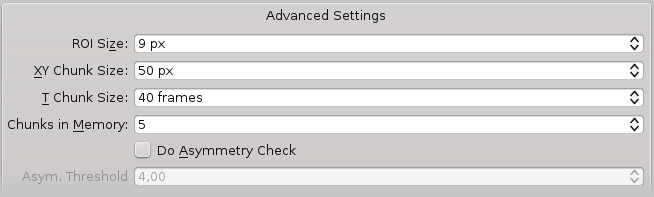
\includegraphics[width = 0.485\textwidth]{pictures/advancedSettingsGui.png}}\hfill
\subfloat[Easy setting widget]{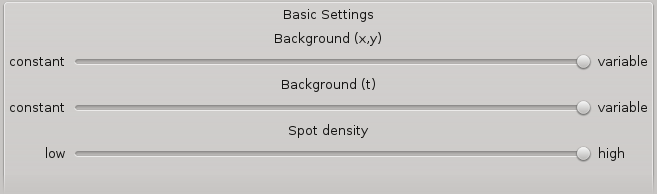
\includegraphics[width = 0.485\textwidth]{pictures/basicSettingsGui1.png}}
	\caption{There are two different ways to set the parameters important for the algorithm. In the picture on the left the standard way of setting parameters can be seen. On the right, there are sliders that can be adjusted between two extrems each. The program sets the value for the parameters in a way to produce the best results for the selected attributes of the data set.}
	\label{guiSettings}	
\end{figure}
\subsection{Result widget}
After the run button at the lower left edge of the input widget was pressed, a new tab opens. In this widget the reconstructed image is shown. At the bottom there is a progress bar that displays at which processing step the program is currently and its progress. Buttons to zoom in and out or to fit the displayed image best into the window. On the lower right there is the stop/save button. It either stops the program if it is still runing or opens a dialog to save the result image and the coordinates of the detection if the program has already been stoped.

\begin{figure}
\subfloat[Input widget]{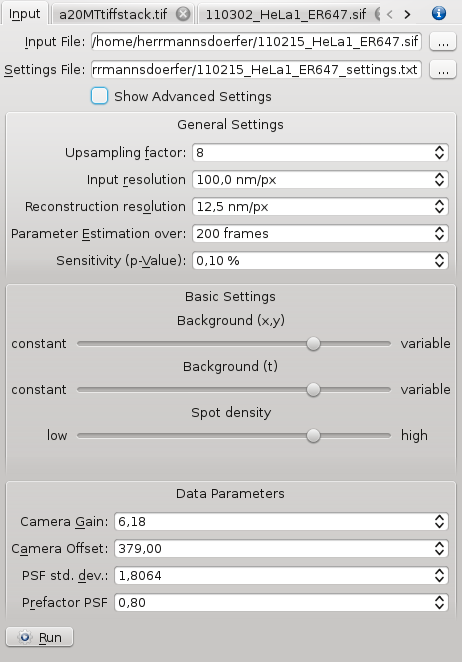
\includegraphics[width = 0.405\textwidth]{pictures/InputWidget.png}}\hfill
\subfloat[Result widget]{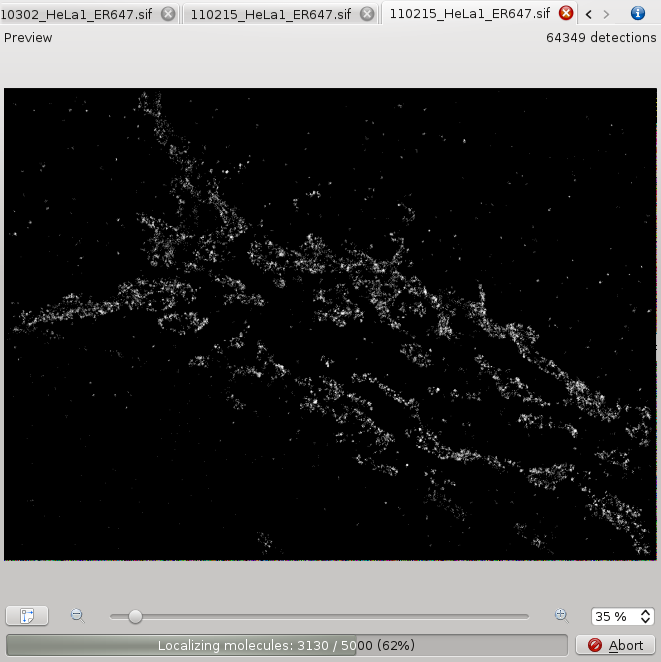
\includegraphics[width = 0.565\textwidth]{pictures/ResultWidget.png}}
	\caption{The new gui design. On the left is the window for selecting input file and parameters show. On the right the result widget showing the procession of a data set in progress.}
	\label{guiWidgets}	
\end{figure}